%________________________________________________%
\section{Introduction}
\label{Sec:Introduction}


%\begin{figure}
%    \centering
%    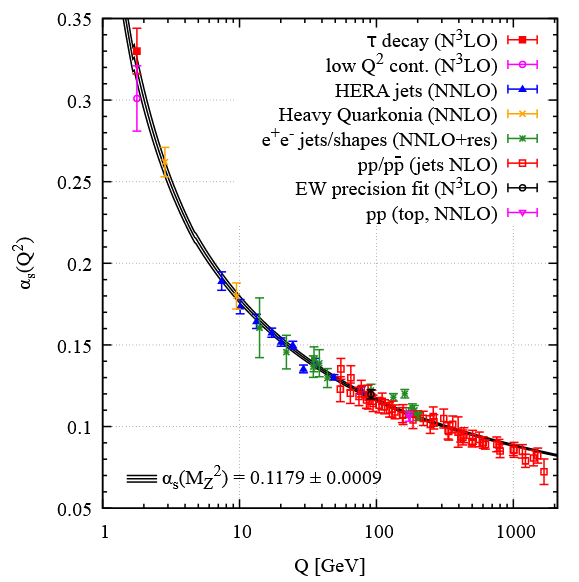
\includegraphics[width=0.5\linewidth]{figures/Introduction-figures/runningCouplingQCD.png}
%    \caption{Summary of measurements of the strong coupling constant $\alpha_{s}$ as a function of the energy scale $Q$. The relative degree of perturbation theory is shown in brackets (NLO: next-to-leading order, NNLO: next-to-next-to-leading order, N$^{3}$LO: next-to-NNLO, NNLO+res: NNLO matched to a resumed calculation). It is evident that the coupling diverges at low energies and perturbation theory starts to break down \cite{PDG} (but text literal from MSc thesis)}
%    \label{fig:secIntro:runningCouplingQCD}
%\end{figure}

The transition from coloured quarks and gluons to colour-neutral, color-singlet hadronic states, commonly referred to as hadronisation, remains one of the central open questions in Quantum Chromodynamics (QCD)~\cite{Andersson:1983ia,Webber:1994zd,Collins:1989gx,Metz:2016swz}. While the production of energetic partons can be described using perturbative techniques, the subsequent confinement of these partons into observable hadrons occurs at energy scales where the strong coupling becomes large and perturbative calculations are no longer applicable. As a result, hadronisation is usually described through phenomenological models that incorporate the essential principles of QCD while relying on experimentally constrained parameters.

The most widely used framework for describing hadronisation in high-energy collisions is the Lund string model~\cite{Andersson:1997xwk,Andersson:2002ap}. In this picture, the colour field between separating colour charges is represented by a string with approximately constant tension. As partons move apart, potential energy is stored in the string until it becomes energetically favourable to produce new quark--antiquark pairs from the vacuum. This consequently fragments the string into smaller pieces that subsequently form hadrons. Implemented in the event generator PYTHIA~\cite{Sjostrand:2014zea}, the Lund string model has been remarkably successful in describing a wide range of observables in lepton and hadron collisions.

The environment of proton--proton collisions, however, introduces additional complexity compared to the simple fragmentation of a single colour-singlet system. Multiple parton interactions (MPI), beam remnants, and overlapping colour fields generate a dense environment of colour fields. To account for these effects, PYTHIA incorporates colour reconnection (CR) mechanisms that allow partons originating from different partonic scatterings to reorganise their colour topology before hadronisation. In the Monash tune, reconnections are performed so as to minimise the overall string length, leading to an improved description of global event properties~\cite{Bierlich:2015rha}. Despite its success, the default string fragmentation framework, even with the inclusion of colour reconnections schemes encounters significant challenges when confronted with measurements of identified-particle production at the Large Hadron Collider (LHC). In particular, the observed enhancement of strange-hadron and baryon production with increasing event activity cannot be fully reproduced by conventional string fragmentation and colour reconnection models~\cite{ALICE:2016fzo}. This has motivated the development of extensions that incorporate additional non-perturbative dynamics.

One such extension is the Beyond-Leading-Colour colour reconnection model~\cite{Christiansen:2015yqa}, which introduces junction topologies. Junctions correspond to Y-shaped colour structures in which three string pieces meet at a common point, providing a natural mechanism for baryon production beyond the traditional diquark picture. The presence of junctions modifies not only baryon yields but also the correlations and balancing of conserved quantum numbers throughout the event. Another extension is the Rope Hadronisation model~\cite{Bierlich:2015rha}, in which overlapping strings combine into colour ropes with an enhanced effective string tension. The larger tension reduces the suppression of, particularly, strange quark and diquark production, leading to increased yields of strange mesons and baryons. More recently, close-packing approaches have been developed to provide a geometrically inspired description of overlapping colour fields and their collective hadronisation.

The importance of these mechanisms has been highlighted by a series of measurements performed at the LHC. In particular, the observation by the ALICE Collaboration of a strong multiplicity-dependent enhancement of strange and multi-strange hadron production in proton--proton collisions~\cite{ALICE:2016fzo} demonstrated that phenomena traditionally associated with larger collision systems are already present in small systems. Similar trends have been observed for baryon-to-meson ratios, indicating that hadron production depends not only on the flavour content of the produced quarks but also on the details of the hadronisation mechanism. Furthermore, ALICE measurements of inclusive $J/\Psi$ production as a function of charged-particle multiplicity revealed a significantly stronger-than-linear increase of the charmonium yield with event activity~\cite{ALICE:2012pet,ALICE:2021zkd}. This observation points to an important role of multiple parton interactions and suggests a non-trivial connection between heavy-flavour production and the global properties of the event. Together, these measurements have established identified-particle production, spanning both light- and heavy-flavour sectors, as a sensitive probe of non-perturbative QCD dynamics and the mechanisms governing hadron formation.

Most studies up to now have focused on light-flavour hadrons, where both the production mechanism and the hadronisation process contribute to the observed final-state particle yields. This complicates the interpretation of baryon-to-meson ratios and quantum-number correlations, since the underlying partonic production rates are themselves difficult to constrain experimentally. Heavy flavour, however, offers a unique opportunity in this respect. Charm and beauty quarks are predominantly produced in hard partonic scatterings at energy scales where perturbative QCD is applicable, and their production cross sections can, in principle, be calculated from first principles. Consequently, heavy-flavour hadrons provide a cleaner laboratory for isolating hadronisation effects from dynamics associated to partonic production.

In this work, we investigate how conserved quantum numbers are balanced during the hadronisation of heavy quarks in proton--proton collisions at LHC energies. Using PYTHIA, we compare the expectations of the Monash tune, junction-based colour reconnection, and close-packing hadronisation models. Starting from produced $c\bar{c}$ and $b\bar{b}$ pairs, we study how the formation of heavy-flavour mesons and baryons is accompanied by balancing particles elsewhere in the event using a two-particle correlations technique described in Section~\ref{Sec:Observables}. The tunes of PYTHIA and the relevant parameters used for ther production of the data samples are described in Section~\ref{Sec:Model}. The results, presented in Section~\ref{Sec:Results}, examine the flavour, baryon-number, and charge correlations associated with identified charm- and beauty-hadron production. They aim to provide new insight into the microscopic mechanisms governing hadronisation and to identify observables capable of discriminating between competing models of non-perturbative QCD.